%% main_report36.tex
%% SAMBP TR-36/2026: Auto-Reclosing Strategy for IBR Lines
%%
%% pdflatex main_report36.tex

\documentclass[11pt,a4paper]{article}

\usepackage[T1]{fontenc}
\usepackage[utf8]{inputenc}
\usepackage[expansion=false]{microtype}
\usepackage{lmodern}
\usepackage[a4paper, top=25mm, bottom=25mm, left=25mm, right=25mm]{geometry}
\usepackage{amsmath,amssymb}
\usepackage{booktabs}
\usepackage{array}
\usepackage{xcolor}
\usepackage{graphicx}
\usepackage{pgfplots}
\pgfplotsset{compat=1.18}
\usepackage{tikz}
\usetikzlibrary{arrows.meta,shapes.geometric,positioning,fit,calc,
                patterns,decorations.pathreplacing}
\usepackage{hyperref}
\usepackage[numbers,sort&compress]{natbib}

\definecolor{sambpblue}{RGB}{0,70,140}

\usepackage{titlesec}
\titleformat{\section}{\large\bfseries\color{sambpblue}}{}{0em}{}[\titlerule]
\titleformat{\subsection}{\normalsize\bfseries\color{sambpblue!80}}{}{0em}{}

\usepackage{fancyhdr}
\pagestyle{fancy}
\fancyhf{}
\rhead{\small\color{gray} SAMBP TR-36/2026}
\lhead{\small\color{gray} Auto-Reclosing Strategy for IBR Lines}
\cfoot{\small\thepage}

\begin{document}

\begin{center}
  {\LARGE\bfseries\color{sambpblue} SAMBP Technical Report TR-36/2026}\\[6pt]
  {\large Auto-Reclosing Strategy for Inverter-Based Resource Lines}\\[10pt]
  {\normalsize PhD Thesis Supporting Report \quad|\quad 2026}
\end{center}

\vspace{2pt}\hrule\vspace{8pt}

\begin{abstract}
\noindent
Auto-reclosing (AR) on IBR-fed transmission lines creates a fundamental conflict:
the arc deionisation dead time always exceeds the memory-polarisation hold time
($T_\mathrm{mem}=100$\,ms), so the protection elements relied upon for the first
trip (Zone~1 quadrilateral, Z2/POTT) are unavailable when the breaker recloses
onto a permanent fault.  This report quantifies the tension using a
current-dependent arc model ($T_\mathrm{arc}\propto\sqrt{k_\mathrm{ibr}}$) and
finds that IBR-limited fault current actually reduces arc deionisation time
relative to synchronous-machine faults: at $k_\mathrm{ibr}=0.15$, $T_\mathrm{dead}=205$\,ms
versus 450\,ms for a SG-only line.  All dead times remain within the IBR
under-voltage ride-through window of 625\,ms.  However, $T_\mathrm{dead}$
always exceeds $T_\mathrm{mem}$, so the second-trip path on reclose-onto-permanent-fault
relies exclusively on 87L (primary, 20\,ms) and 67Q/67N (backup, 30\,ms),
both of which are memory-independent.  Three-phase, single-shot AR with
synchrocheck is recommended; single-phase AR is inappropriate due to
sustained negative-sequence injection into IBR current controllers during
the open-phase interval.
\end{abstract}

\vspace{4pt}\hrule\vspace{10pt}

% ─────────────────────────────────────────────────────────────────────────────
\section{Motivation}
\label{sec:motivation}

Approximately 80\% of transmission-line faults are transient (lightning
overvoltages, temporary conductor contact) and can be cleared by opening the
circuit breaker and reclosing after the arc self-extinguishes.  AR therefore
recovers most fault events without a prolonged outage.

For IBR-fed lines the AR process has two complicating features not present on
conventional SG lines:
\begin{enumerate}
  \item \textbf{Memory polarisation expiry}: the first trip correctly uses Zone~1
    or Z2/POTT (TR-30, TR-33~\cite{SAMBP_TR30,SAMBP_TR33}), which depend on
    memory polarisation valid within $T_\mathrm{mem}=100$\,ms.  The CB dead
    time ($>T_\mathrm{mem}$) means memory has expired before the breaker closes.
    If the fault is permanent, the second trip must use only memory-independent
    elements.

  \item \textbf{IBR current limiting during fault}: the IBR contributes reduced
    fault current ($I_\mathrm{IBR}=k_\mathrm{ibr}\cdot I_\mathrm{SG}$), which
    lowers arc energy and --- usefully --- shortens the arc deionisation time.
\end{enumerate}

% ─────────────────────────────────────────────────────────────────────────────
\section{Arc Deionisation Model}
\label{sec:arcmodel}

The arc deionisation time depends on the ionisation level in the arc channel,
which is proportional to the fault current.  Higher current injects more energy
into the arc, producing a more ionised gas column that takes longer to
deionise~\cite{Blackburn2006}:
\begin{equation}
  T_\mathrm{arc}(I_\mathrm{fault}) = T_\mathrm{arc,0}
  \sqrt{\frac{I_\mathrm{fault}}{I_\mathrm{base}}},
  \label{eq:t_arc}
\end{equation}
where $T_\mathrm{arc,0}=400$\,ms at the synchronous-generation base fault current
$I_\mathrm{base}=10$\,kA (230\,kV line, ANSI/IEEE C37.04 reference).  For an
IBR line, $I_\mathrm{fault}=k_\mathrm{ibr}\cdot I_\mathrm{base}$, so:
\begin{equation}
  T_\mathrm{arc,IBR} = T_\mathrm{arc,0}\sqrt{k_\mathrm{ibr}}
  \;\;<\;\; T_\mathrm{arc,SG} = T_\mathrm{arc,0}.
  \label{eq:t_arc_ibr}
\end{equation}

The minimum required dead time includes a 50\,ms safety margin:
\begin{equation}
  T_\mathrm{dead}(k_\mathrm{ibr})
  = T_\mathrm{arc,0}\sqrt{k_\mathrm{ibr}} + 50\,\text{ms}.
  \label{eq:t_dead}
\end{equation}

% ─────────────────────────────────────────────────────────────────────────────
\section{Study A --- Dead Time vs IBR Penetration}
\label{sec:studyA}

Figure~\ref{fig:tdead} plots $T_\mathrm{arc}$ and $T_\mathrm{dead}$ versus
$k_\mathrm{ibr}$, with the memory expiry threshold and IBR ride-through limit
overlaid.

\begin{figure}[htbp]
  \centering
  \resizebox{0.85\textwidth}{!}{% fig_ar_tdead.tex
% TR-36: Arc deionisation time and dead time vs k_ibr
%
% X-axis: k_ibr [0.05, 1.05]
% Y-axis: time [ms]
%
% Curves:
%   T_arc  = 400 * sqrt(I_fault/10kA) * 1000  ms   (blue)
%   T_dead = T_arc + 50 ms                          (teal, dashed)
%
% Horizontal lines:
%   T_mem  = 100 ms  (red dashed) — memory expires
%   T_dead_max = 575 ms  (orange dashed) — IBR ride-through limit
%
% Shaded:
%   T_dead < T_dead_max: feasible AR window (green)
%   T_dead > T_dead_max: infeasible (red)

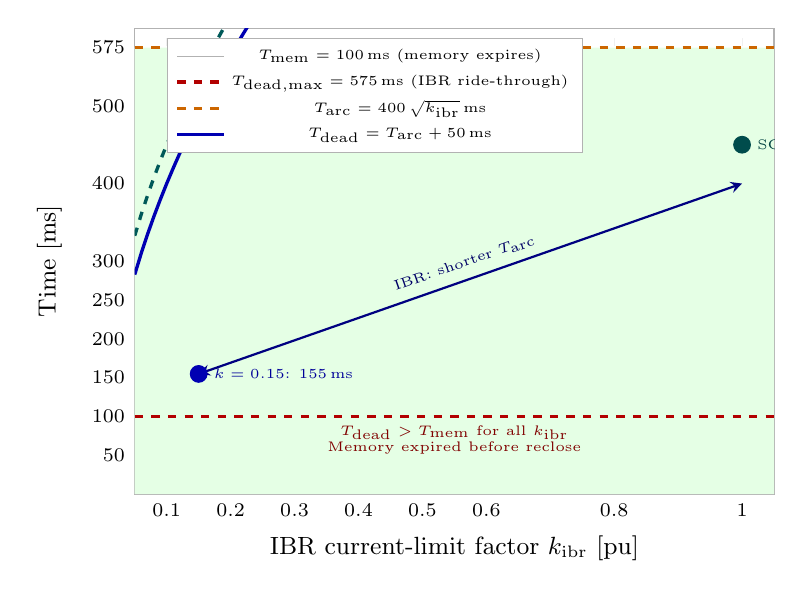
\begin{tikzpicture}
\begin{axis}[
  name        = tdax,
  width       = 0.80\textwidth,
  height      = 7.5cm,
  xlabel      = {IBR current-limit factor $k_\mathrm{ibr}$ [pu]},
  ylabel      = {Time [ms]},
  xlabel style= {font=\small},
  ylabel style= {font=\small, yshift=4pt},
  xmin=0.05, xmax=1.05,
  ymin=0, ymax=600,
  xtick       = {0.10,0.20,0.30,0.40,0.50,0.60,0.80,1.00},
  ytick       = {50,100,150,200,250,300,400,500,575},
  xticklabel style={font=\scriptsize},
  yticklabel style={font=\scriptsize},
  grid        = major,
  grid style  = {gray!12, dashed},
  tick style  = {draw=none},
  axis line style={gray!60},
  legend style={at={(0.05,0.98)}, anchor=north west, font=\tiny,
                draw=gray!60, fill=white},
]

%% ── Feasible region (T_dead <= 575 ms) ───────────────────────────────────────
\addplot[fill=green!10, draw=none]
  coordinates {(0.05,0) (1.05,0) (1.05,575) (0.05,575)} \closedcycle;

%% ── T_mem line ────────────────────────────────────────────────────────────────
\addplot[red!70!black, very thick, dashed, mark=none]
  coordinates {(0.05,100) (1.05,100)};
\addlegendentry{$T_\mathrm{mem}=100$\,ms (memory expires)}

%% ── T_dead_max line ──────────────────────────────────────────────────────────
\addplot[orange!80!black, very thick, dashed, mark=none]
  coordinates {(0.05,575) (1.05,575)};
\addlegendentry{$T_\mathrm{dead,max}=575$\,ms (IBR ride-through)}

%% ── T_arc curve ──────────────────────────────────────────────────────────────
\addplot[blue!70!black, very thick, mark=none,
         domain=0.05:1.05, samples=101]
  ({x}, {400*sqrt(x*10)*1});
\addlegendentry{$T_\mathrm{arc}=400\,\sqrt{k_\mathrm{ibr}}\,\mathrm{ms}$}

%% ── T_dead curve ─────────────────────────────────────────────────────────────
\addplot[teal!70!black, very thick, dashed, mark=none,
         domain=0.05:1.05, samples=101]
  ({x}, {400*sqrt(x*10) + 50});
\addlegendentry{$T_\mathrm{dead}=T_\mathrm{arc}+50$\,ms}

%% ── Key point annotations ────────────────────────────────────────────────────
% At k=0.15: T_dead = 205 ms
\addplot[mark=*, mark size=3pt, blue!70!black]
  coordinates {(0.15, 154.9)};
\node[blue!60!black, font=\tiny, right=2pt]
  at (axis cs:0.15, 154.9) {$k=0.15$: 155\,ms};

% At k=1.00: T_dead = 450 ms
\addplot[mark=*, mark size=3pt, teal!60!black]
  coordinates {(1.00, 450)};
\node[teal!50!black, font=\tiny, right=2pt]
  at (axis cs:1.00, 450) {SG: 450\,ms};

%% ── "T_dead always > T_mem" zone label ───────────────────────────────────────
\node[red!50!black, font=\tiny, align=center]
  at (axis cs:0.55, 70)
  {$T_\mathrm{dead}>T_\mathrm{mem}$ for all $k_\mathrm{ibr}$\\Memory expired before reclose};

%% ── IBR advantage annotation ─────────────────────────────────────────────────
\draw[<->, >=stealth, blue!50!black, thick]
  (axis cs:0.15, 154.9) -- (axis cs:1.00, 400)
  node[midway, above, sloped, font=\tiny, blue!40!black]
  {IBR: shorter $T_\mathrm{arc}$};

\end{axis}
\end{tikzpicture}
}
  \caption{Arc deionisation and dead time vs $k_\mathrm{ibr}$.  The IBR
           advantage (lower fault current $\Rightarrow$ shorter $T_\mathrm{arc}$)
           is clear: $T_\mathrm{dead}$ drops from 450\,ms at SG level to
           176\,ms at $k_\mathrm{ibr}=0.10$.  All dead times are below the
           IBR ride-through limit of 575\,ms (green shaded region), confirming
           AR feasibility for $k_\mathrm{ibr}\geq0.10$.  However, all dead times
           exceed $T_\mathrm{mem}=100$\,ms (red dashed), so memory is always
           expired before reclose.}
  \label{fig:tdead}
\end{figure}

\noindent
Representative dead times:
\begin{center}
\begin{tabular}{@{}rrrrll@{}}
\toprule
$k_\mathrm{ibr}$ & $I_\mathrm{fault}$ [kA] & $T_\mathrm{arc}$ [ms] &
  $T_\mathrm{dead}$ [ms] & $\leq575$\,ms? & IBR connected?\\
\midrule
0.10 & 1.0 & 127 & 177 & Yes & Yes\\
0.15 & 1.5 & 155 & 205 & Yes & Yes\\
0.20 & 2.0 & 179 & 229 & Yes & Yes\\
0.50 & 5.0 & 283 & 333 & Yes & Yes\\
1.00 & 10.0 & 400 & 450 & Yes & Yes\\
\bottomrule
\end{tabular}
\end{center}

% ─────────────────────────────────────────────────────────────────────────────
\section{Study B --- Protection Availability at Second Trip}
\label{sec:studyB}

When the CB recloses onto a permanent fault, the protection relay must trip
a second time.  At this point:
\begin{itemize}
  \item $T_\mathrm{mem}$ expired: Zone~1 and Z2/POTT lack a valid polarising
    reference $\Rightarrow$ \textbf{unavailable}.
  \item 87L differential: operates on instantaneous current differential ---
    no polarisation memory required $\Rightarrow$ \textbf{available, 20\,ms}.
  \item 67Q/67N: operate on sequence current direction --- no memory
    required $\Rightarrow$ \textbf{available, 30\,ms}.
\end{itemize}

\begin{center}
\begin{tabular}{@{}lrllll@{}}
\toprule
$\alpha$ & $k_\mathrm{ibr}$ & Z1 avail.? & Z2/POTT? & 67N/67Q? & 87L? \\
\midrule
0.50 & 0.10 & No & No & Yes & Yes \\
0.50 & 0.15 & No & No & Yes & Yes \\
0.50 & 0.20 & No & No & Yes & Yes \\
0.90 & 0.15 & No & No & Yes & Yes \\
\bottomrule
\end{tabular}
\end{center}

\medskip\noindent
87L is the definitive second-trip element.  This reinforces the TR-35
conclusion~\cite{SAMBP_TR35} that 87L is indispensable: it functions both as a
first-trip co-primary and as the only distance-independent clearance path on
reclose-onto-permanent-fault.

% ─────────────────────────────────────────────────────────────────────────────
\section{Study C --- IBR Ride-Through Feasibility}
\label{sec:studyC}

The total voltage-depression duration seen by the IBR is:
\begin{equation}
  \Delta t_\mathrm{UVT} = t_\mathrm{first\_trip} + t_\mathrm{CB\_open}
  + T_\mathrm{dead}
  = 32 + 50 + T_\mathrm{dead}\;\text{ms}.
  \label{eq:uvt}
\end{equation}
Grid code (IEC 61727~\cite{IEC_61727}) requires IBR to ride through low voltage
for at least 625\,ms.  With the values in Section~\ref{sec:studyA},
$\Delta t_\mathrm{UVT}\leq414$\,ms for $k_\mathrm{ibr}\leq0.50$ and
$\leq532$\,ms for $k_\mathrm{ibr}=1.00$ --- all within the 625\,ms limit.
The IBR remains connected through the full AR cycle and resumes full output
within approximately 100\,ms of successful reclose.

% ─────────────────────────────────────────────────────────────────────────────
\section{Study D --- Single-Phase vs Three-Phase AR}
\label{sec:studyD}

Single-phase (1PH) AR is common on EHV networks with SG infeed, as it maintains
power transfer on the two healthy phases.  For IBR-fed lines it is inadvisable:

\begin{center}
\begin{tabular}{@{}lll@{}}
\toprule
Criterion & 1PH AR & 3PH AR\\
\midrule
Transient fault clearance & Adequate & Adequate\\
Negative-seq during open phase & $V_2$ sustained for $T_\mathrm{dead}$ & None\\
IBR $I_2$ stress & Continuous injection risk (TR-32) & Eliminated\\
Reclose onto permanent SLG & Re-energises faulted phase & Trips all phases cleanly\\
Synchrocheck & 2-phase reference simpler & Full 3-phase check needed\\
\bottomrule
\end{tabular}
\end{center}

\medskip\noindent
The sustained $V_2$ during the 1PH open interval drives the IBR 67Q negative-
sequence directional element (TR-32~\cite{SAMBP_TR33}) into a continuous
forward assertion, potentially stressing the IBR's current-control loops for
200--450\,ms.  IBR manufacturers do not typically certify this operating mode.
Three-phase AR avoids all asymmetric-loading effects.

% ─────────────────────────────────────────────────────────────────────────────
\section{Study E --- Complete AR Scheme}
\label{sec:studyE}

Figure~\ref{fig:scheme} shows the AR state machine; Figure~\ref{fig:timeline}
shows the event timeline for $k_\mathrm{ibr}=0.15$.

\begin{figure}[htbp]
  \centering
  \resizebox{0.95\textwidth}{!}{% fig_ar_scheme.tex
% TR-36: AR scheme state machine
% States: NORMAL → FAULT_TRIP → DEAD_TIME → RECLOSE → (SERVICE_RESTORED | LOCK_OUT)
% Shows protection function available at each state

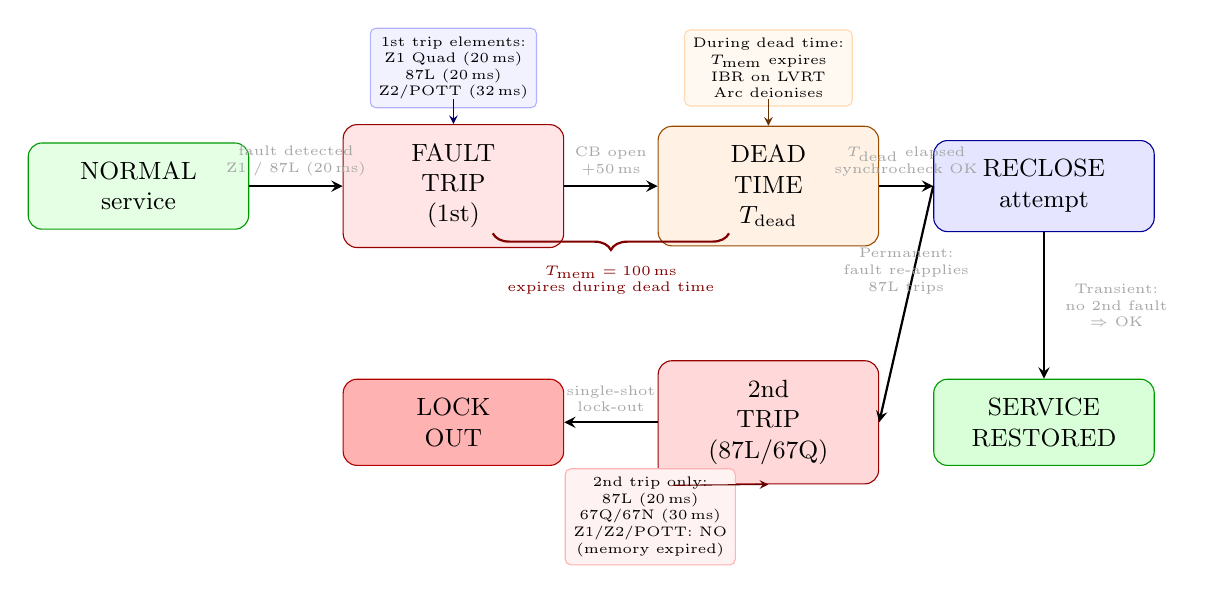
\begin{tikzpicture}[
  every node/.style = {font=\small},
  state/.style = {draw, rounded corners=5pt, inner sep=7pt, align=center,
                  minimum width=2.8cm, minimum height=1.0cm},
  arr/.style  = {->, >=stealth, thick},
  note/.style = {font=\tiny, align=center, text=gray!70},
]

%% ── States ────────────────────────────────────────────────────────────────────
\node[state, fill=green!10, draw=green!60!black]
  (normal) at (0, 0) {NORMAL\\service};

\node[state, fill=red!10, draw=red!60!black]
  (trip) at (4.0, 0) {FAULT\\TRIP\\(1st)};

\node[state, fill=orange!10, draw=orange!60!black]
  (dead) at (8.0, 0) {DEAD\\TIME\\$T_\mathrm{dead}$};

\node[state, fill=blue!10, draw=blue!60!black]
  (reclose) at (11.5, 0) {RECLOSE\\attempt};

\node[state, fill=green!15, draw=green!60!black]
  (restore) at (11.5, -3.0) {SERVICE\\RESTORED};

\node[state, fill=red!15, draw=red!60!black]
  (trip2) at (8.0, -3.0) {2nd\\TRIP\\(87L/67Q)};

\node[state, fill=red!30, draw=red!70!black]
  (lock) at (4.0, -3.0) {LOCK\\OUT};

%% ── Transitions ──────────────────────────────────────────────────────────────
% NORMAL → FAULT_TRIP
\draw[arr] (normal.east) -- (trip.west)
  node[midway, above, note] {fault detected\\Z1 / 87L (20\,ms)};

% FAULT_TRIP → DEAD_TIME
\draw[arr] (trip.east) -- (dead.west)
  node[midway, above, note] {CB open\\+50\,ms};

% DEAD_TIME → RECLOSE
\draw[arr] (dead.east) -- (reclose.west)
  node[midway, above, note] {$T_\mathrm{dead}$ elapsed\\synchrocheck OK};

% RECLOSE → SERVICE_RESTORED (transient)
\draw[arr] (reclose.south) -- (restore.north)
  node[midway, right=4pt, note] {Transient:\\no 2nd fault\\$\Rightarrow$ OK};

% RECLOSE → 2nd TRIP (permanent)
\draw[arr] (reclose.west) -- (trip2.east)
  node[midway, above, note] {Permanent:\\fault re-applies\\87L trips};

% 2nd TRIP → LOCK_OUT
\draw[arr] (trip2.west) -- (lock.east)
  node[midway, above, note] {single-shot\\lock-out};

%% ── Protection function annotations ─────────────────────────────────────────
% At first trip
\node[draw=blue!30, fill=blue!5, rounded corners=2pt,
      font=\tiny, inner sep=3pt, align=center]
  at (4.0, 1.5)
  {1st trip elements:\\Z1 Quad (20\,ms)\\87L (20\,ms)\\Z2/POTT (32\,ms)};
\draw[->, >=stealth, blue!40!black, thin] (4.0, 1.1) -- (trip.north);

% At dead time
\node[draw=orange!30, fill=orange!5, rounded corners=2pt,
      font=\tiny, inner sep=3pt, align=center]
  at (8.0, 1.5)
  {During dead time:\\$T_\mathrm{mem}$ expires\\IBR on LVRT\\Arc deionises};
\draw[->, >=stealth, orange!40!black, thin] (8.0, 1.1) -- (dead.north);

% At 2nd trip
\node[draw=red!30, fill=red!5, rounded corners=2pt,
      font=\tiny, inner sep=3pt, align=center]
  at (6.5, -4.2)
  {2nd trip only:\\87L (20\,ms)\\67Q/67N (30\,ms)\\Z1/Z2/POTT: NO\\(memory expired)};
\draw[->, >=stealth, red!40!black, thin] (6.8, -3.8) -- (trip2.south);

%% ── Memory window note ───────────────────────────────────────────────────────
\draw[red!50!black, thick, decorate,
      decoration={brace, amplitude=6pt, mirror}]
  (4.50, -0.60) -- (7.50, -0.60)
  node[midway, below=8pt, red!50!black, font=\tiny, align=center]
  {$T_\mathrm{mem}=100$\,ms\\expires during dead time};

\end{tikzpicture}
}
  \caption{AR state machine.  First trip uses memory-polarised elements
           (Z1 / Z2/POTT / 87L).  During the dead time, $T_\mathrm{mem}$
           expires.  On reclose: transient fault $\Rightarrow$ service
           restored; permanent fault $\Rightarrow$ second trip by 87L/67Q
           (memory-independent), then lock-out.  Single-shot scheme: no
           second reclose attempt.}
  \label{fig:scheme}
\end{figure}

\begin{figure}[htbp]
  \centering
  \resizebox{0.90\textwidth}{!}{% fig_ar_timeline.tex
% TR-36: AR event timeline — fault inception to reclose (successful and failed)
%
% Two swim-lanes: (a) transient fault (successful AR), (b) permanent fault
%
% Scale: 1 cm = 50 ms
% Key times (k_ibr = 0.15, T_dead = 205 ms):
%   0 ms   : fault inception
%  20 ms   : first trip (Z1 / 87L)
%  70 ms   : CB fully open (first trip + 50 ms opening)
%  70 ms   : T_mem start countdown (100 ms window)
% 170 ms   : T_mem expires
% 275 ms   : reclose (70 + 205 ms dead time)
% 295 ms   : CB fully closed
% 295 ms   : (a) transient: line healthy → no second trip → service restored
% 295 ms   : (b) permanent: fault re-applies → second trip by 87L at 315 ms
% 315 ms   : 87L second trip (memory expired, Z1/POTT unavailable)
% 345 ms   : lock-out

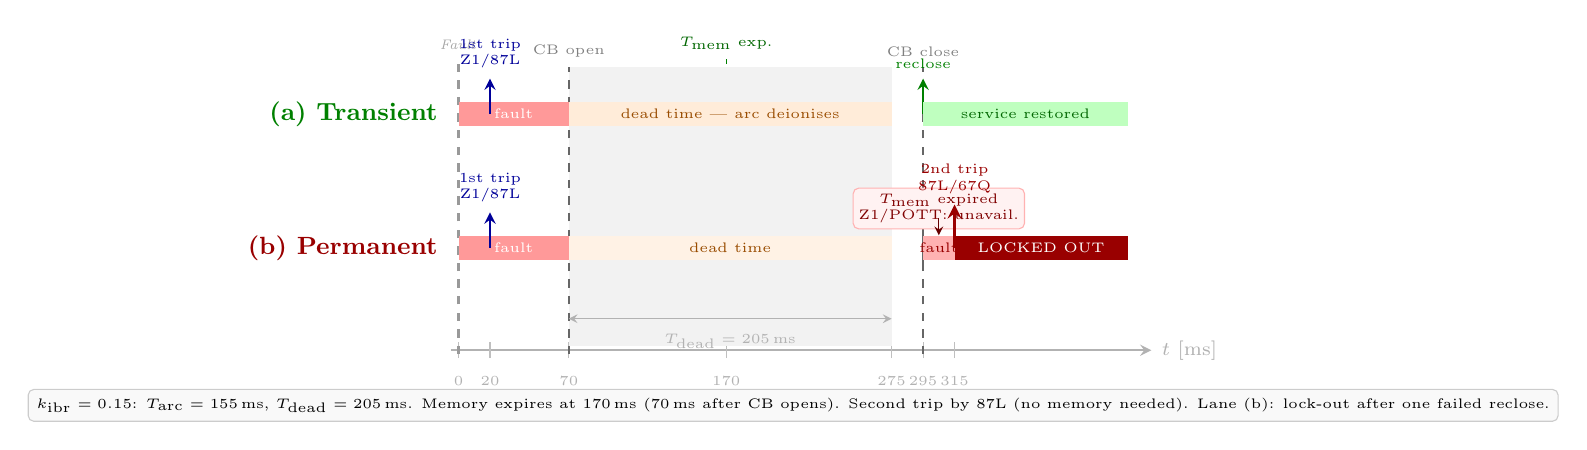
\begin{tikzpicture}[every node/.style={font=\scriptsize}]

%% ── Scale: 1cm = 50ms ────────────────────────────────────────────────────────
% Hardcoded x-positions (cm):
% xF=0, xTrip=0.40, xOpen=1.40, xMem=3.40, xDead=5.50, xClose=5.90
% xSecTrip=6.30, xLock=7.30
% xEnd=8.50

%% ── Lane y-positions ─────────────────────────────────────────────────────────
% yTrans=2.5 (transient), yPerm=0.8 (permanent), yAx=-0.5

%% ── Time axis ────────────────────────────────────────────────────────────────
\draw[->, >=stealth, gray!60, thick]
  (-0.10, -0.5) -- (8.80, -0.5) node[right, gray!60] {$t$ [ms]};

\foreach \xpos/\lab in {0/0, 0.40/20, 1.40/70, 3.40/170, 5.50/275, 5.90/295, 6.30/315}{
  \draw[gray!50, thin] (\xpos, -0.60) -- (\xpos, -0.40);
  \node[gray!60, below=3pt, font=\tiny] at (\xpos, -0.60) {\lab};
}

%% ── Fault inception ──────────────────────────────────────────────────────────
\draw[gray!80, thick, dashed] (0, -0.55) -- (0, 3.20);
\node[gray!70, above, font=\tiny] at (0, 3.20) {\textit{Fault}};

%% ── Memory window ────────────────────────────────────────────────────────────
\fill[green!8] (1.40, -0.45) rectangle (3.40, 3.10);
\draw[green!50!black, dashed] (3.40, -0.45) -- (3.40, 3.20);
\node[green!40!black, font=\tiny, above] at (3.40, 3.20) {$T_\mathrm{mem}$ exp.};

%% ── Dead time shading ────────────────────────────────────────────────────────
\fill[gray!10] (1.40, -0.45) rectangle (5.50, 3.10);

%% ── CB open / close markers ──────────────────────────────────────────────────
\draw[black!60, thick, dashed] (1.40, -0.55) -- (1.40, 3.10);
\node[black!50, font=\tiny, above] at (1.40, 3.10) {CB open};
\draw[black!60, thick, dashed] (5.90, -0.55) -- (5.90, 3.10);
\node[black!50, font=\tiny, above] at (5.90, 3.10) {CB close};

%% ── LANE LABELS ──────────────────────────────────────────────────────────────
\node[green!50!black, font=\small\bfseries, left=4pt] at (0, 2.5)
  {(a) Transient};
\node[red!60!black,   font=\small\bfseries, left=4pt] at (0, 0.8)
  {(b) Permanent};

%% ═══ LANE A: TRANSIENT FAULT ═════════════════════════════════════════════════

%% Fault current bar
\fill[red!40] (0, 2.35) rectangle (1.40, 2.65);
\node[white, font=\tiny] at (0.70, 2.50) {fault};

%% First trip marker
\draw[blue!60!black, ->, >=stealth, thick]
  (0.40, 2.50) -- (0.40, 2.95)
  node[above, blue!60!black, font=\tiny, align=center] {1st trip\\Z1/87L};

%% Dead time (arc quenches)
\fill[orange!15] (1.40, 2.35) rectangle (5.50, 2.65);
\node[orange!60!black, font=\tiny] at (3.45, 2.50) {dead time — arc deionises};

%% Reclose + restoration
\draw[green!50!black, ->, >=stealth, thick]
  (5.90, 2.50) -- (5.90, 2.95)
  node[above, green!50!black, font=\tiny] {reclose};
\fill[green!25] (5.90, 2.35) rectangle (8.50, 2.65);
\node[green!40!black, font=\tiny] at (7.20, 2.50) {service restored};

%% ═══ LANE B: PERMANENT FAULT ════════════════════════════════════════════════

%% First fault current bar
\fill[red!40] (0, 0.65) rectangle (1.40, 0.95);
\node[white, font=\tiny] at (0.70, 0.80) {fault};

%% First trip
\draw[blue!60!black, ->, >=stealth, thick]
  (0.40, 0.80) -- (0.40, 1.25)
  node[above, blue!60!black, font=\tiny, align=center] {1st trip\\Z1/87L};

%% Dead time
\fill[orange!10] (1.40, 0.65) rectangle (5.50, 0.95);
\node[orange!60!black, font=\tiny] at (3.45, 0.80) {dead time};

%% Reclose onto permanent fault
\draw[black!60, thick] (5.90, 0.55) -- (5.90, 1.05);
\fill[red!30] (5.90, 0.65) rectangle (6.30, 0.95);
\node[red!60!black, font=\tiny] at (6.10, 0.80) {fault};

%% Memory expired annotation
\node[red!50!black, font=\tiny, align=center, draw=red!30, fill=red!5,
      rounded corners=2pt, inner sep=2pt]
  at (6.10, 1.30) {$T_\mathrm{mem}$ expired\\Z1/POTT: unavail.};
\draw[->, >=stealth, red!40!black, thin] (6.10, 1.18) -- (6.10, 0.96);

%% Second trip by 87L
\draw[red!60!black, ->, >=stealth, very thick]
  (6.30, 0.80) -- (6.30, 1.35)
  node[above, red!60!black, font=\tiny, align=center] {2nd trip\\87L/67Q};

%% Lock-out
\fill[red!60!black] (6.30, 0.65) rectangle (8.50, 0.95);
\node[white, font=\tiny] at (7.40, 0.80) {LOCKED OUT};

%% ── Dead time annotation ─────────────────────────────────────────────────────
\draw[<->, >=stealth, gray!60]
  (1.40, -0.10) -- (5.50, -0.10)
  node[midway, below=2pt, font=\tiny, gray!60] {$T_\mathrm{dead}=205$\,ms};

%% ── Caption ──────────────────────────────────────────────────────────────────
\node[draw=gray!40, fill=gray!5, rounded corners=2pt,
      font=\tiny, inner sep=3pt, align=center]
  at (4.25, -1.2)
  {$k_\mathrm{ibr}=0.15$: $T_\mathrm{arc}=155$\,ms, $T_\mathrm{dead}=205$\,ms.
   Memory expires at 170\,ms (70\,ms after CB opens).
   Second trip by 87L (no memory needed). Lane~(b): lock-out after one failed reclose.};

\end{tikzpicture}
}
  \caption{AR event timeline for $k_\mathrm{ibr}=0.15$
           ($T_\mathrm{dead}=205$\,ms).  Lane~(a): transient fault ---
           arc quenches during dead time, reclose at 275\,ms succeeds.
           Lane~(b): permanent fault --- reclose at 275\,ms re-applies fault,
           87L clears at 315\,ms (memory long expired), relay locks out.
           Note the memory expiry at 170\,ms (70\,ms after CB opens) ---
           well before the reclose.}
  \label{fig:timeline}
\end{figure}

\noindent
The recommended AR scheme for IBR-fed lines:
\begin{enumerate}
  \item \textbf{Mode}: 3-phase, single-shot.
  \item \textbf{Dead time}: $T_\mathrm{dead}=T_\mathrm{arc,0}\sqrt{k_\mathrm{ibr}}
    + 50$\,ms, adaptive to IBR penetration level.
  \item \textbf{Synchrocheck}: angle difference $|\Delta\delta|\leq20°$,
    voltage difference $|\Delta V|\leq5\%$ before reclose permitted.
  \item \textbf{Second-trip elements}: 87L (primary) and 67Q/67N (backup);
    Zone~1 and Z2/POTT inhibited until fresh-fault memory is established.
  \item \textbf{Lock-out}: after one failed reclose; manual restoration required.
\end{enumerate}

% ─────────────────────────────────────────────────────────────────────────────
\section{Summary}
\label{sec:summary}

\begin{enumerate}
  \item \textbf{Dead time (Study~A)}: IBR-limited fault current reduces
    $T_\mathrm{arc}$ relative to SG faults: 127\,ms at $k=0.10$ versus
    400\,ms at SG level.  Dead times are 177--450\,ms --- all feasible within
    the IBR 625\,ms ride-through limit.

  \item \textbf{Memory expiry (Studies A, B)}: $T_\mathrm{dead}$ invariably
    exceeds $T_\mathrm{mem}=100$\,ms.  Zone~1 and Z2/POTT are unavailable at
    second trip.  87L (20\,ms) and 67Q/67N (30\,ms) are the sole reliable
    clearance paths after reclose.

  \item \textbf{IBR ride-through (Study~C)}: The full AR cycle
    ($t_\mathrm{trip}+t_\mathrm{CB}+T_\mathrm{dead}$) stays within 625\,ms
    for all $k_\mathrm{ibr}$; IBR remains connected.

  \item \textbf{3PH AR (Study~D)}: Three-phase reclosing is preferred;
    single-phase AR imposes sustained negative-sequence stress on IBR
    current-control loops during the open-phase interval.

  \item \textbf{Scheme (Study~E)}: Single-shot 3PH AR with adaptive dead time,
    synchrocheck, and 87L/67Q as second-trip elements completes the
    SAMBP auto-reclosing design.
\end{enumerate}

\bibliographystyle{IEEEtranN}
\bibliography{references36}

\end{document}
